\documentclass[12pt]{article}

\usepackage[margin = .8in]{geometry}
\usepackage{amsmath}
\usepackage{graphicx}
\usepackage{multicol, enumerate}

\usepackage{adjustbox}

\usepackage{fancyhdr}
\pagestyle{fancy}

\lhead{Math F113X: Numbers and Society}
\rhead{Date: \hspace{1in}}

\usepackage{tikz}
\usetikzlibrary{calc,trees,positioning,arrows,fit,shapes,through}
\usetikzlibrary{patterns}

\usetikzlibrary{decorations.markings}
\usetikzlibrary{arrows}

\usepackage{pgfplots}

\usepackage{longtable}
\usepackage{tabularx}

\newcommand{\ds}{\displaystyle}
\newcommand{\ans}[1][1in]{\rule{#1}{.5pt}}

\newcommand{\points}[1]{(#1 points.)}		% Trying to be lazy.

\usepackage{array}
\newcolumntype{L}[1]{>{\raggedright\let\newline\\\arraybackslash\hspace{0pt}}m{#1}}
\newcolumntype{C}[1]{>{\centering\let\newline\\\arraybackslash\hspace{0pt}}m{#1}}
\newcolumntype{R}[1]{>{\raggedleft\let\newline\\\arraybackslash\hspace{0pt}}m{#1}}
\newcommand{\red}[1]{\textcolor{red}{#1}}

\newcommand{\be}{\begin{enumerate}}
\newcommand{\ee}{\end{enumerate}}

%\topmargin -1in
%\textheight 9.5in
%\oddsidemargin -0.3in
%\evensidemargin \oddsidemargin
%\pagestyle{empty}
%%\marginparwidth 0.5in
%\textwidth 7in
%\parindent 0in

%--------------------------------------------------------------------------------------------------------------------------------------------------------------------------
%						Document
%--------------------------------------------------------------------------------------------------------------------------------------------------------------------------


\begin{document}
%\pagestyle{fancy}
\begin{center}
{\Large  Worksheet 10 (Graph Theory 2): Shortest distance on a graph}
\end{center}



\noindent \textbf{Group Names:} \hrulefill \\
%-------------------------------------------------------------------------------------------------------------
%						Assignment
%-----------------------------------------------------------------------------------------------------
\begin{enumerate}
\item Use Dijkstra's Algorithm to determine the shortest (weighted) distance between vertex $S$ and each other vertex in the graph. Break any ties by choosing the vertex that comes earlier in the alphabet.

Keep track of the steps of the algorithm in the table to the right of the graph, and then fill in the final shortest distances between $S$ and each other vertex below.

\begin{adjustbox}{valign=t,minipage={.4\textwidth}}
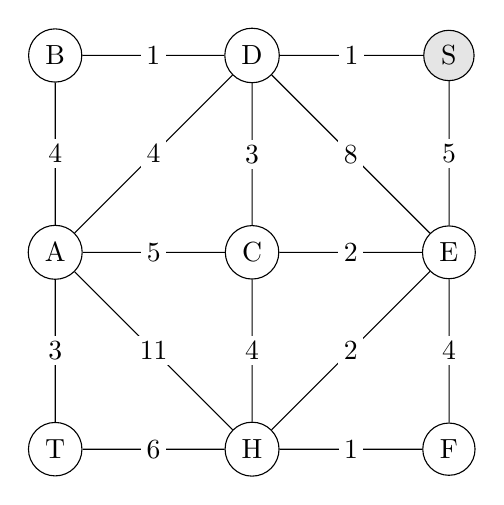
\begin{tikzpicture}[scale=2.5, lbl/.style={midway, fill=white, inner sep = 2pt}]
\node[draw, circle] (A) at (1,0) {A} ;
\node[draw, circle] (B) at (1,1) {B} ;
\node[draw, circle] (C) at (2,0) {C} ;
\node[draw, circle] (D) at (2,1) {D} ;
\node[draw, circle] (E) at (3,0) {E} ;
\node[draw, circle, fill=gray!20] (F) at (3,1) {S} ;
\node[draw, circle] (H) at (2,-1) {H} ;
\node[draw, circle] (I) at (3,-1) {F} ;
\node[draw, circle] (T) at (1,-1) {T};

\draw (A) -- node[lbl]{4}(B)  -- node[lbl]{1} (D) -- node[lbl]{3}(C) -- node[lbl]{2} (E) -- node[lbl]{5}(F);
\draw (A) -- node[lbl] {5} (C)  -- node[lbl] {4}(H)  -- node[lbl] {1} (I) -- node[lbl] {4} (E) ;
\draw (D) -- node[lbl]{1} (F) ;\draw (H) -- node[lbl]{11} (A);
\draw (E) -- node[lbl]{2}(H) ;\draw (D) -- node[lbl]{4}(A);
\draw (D) -- node[lbl] {8} (E);
\draw (A) -- node[lbl]{3} (T);
\draw (T) -- node[lbl]{6}(H);
\end{tikzpicture}
\end{adjustbox}
%\hfill
\begin{adjustbox}{valign=t,minipage={.25\textwidth}}

\begin{tabular}{ c | c | p{2in}}
Explored? & vertices & tentative distances\\ \hline
& \\
& \\
& \\& \\& \\& \\& \\& \\& \\% \\& \\& \\
 \end{tabular}


\end{adjustbox}


\vspace{1cm}

\begin{adjustbox}{valign=t,minipage={.5\textwidth}}
{
 \begin{tabular}{c | c}
vertex &  distance from $S$\\
\hline
S & \\ 
A & \\ 
B & \\
C & \\ D & \\ E & \\ F & \\ H & \\ T & \\
\end{tabular}
}
\end{adjustbox}

%\bigskip
\vfill

\hfill{...continued on the back side}

\newpage

\item We can also use Dijkstra's algorithm to find the shortest distance between two vertices in a graph that does not have weights on the edges, by assuming all of the weights are 1. As usual, break ties alphabetically.

\begin{adjustbox}{valign=t,minipage={.4\textwidth}}
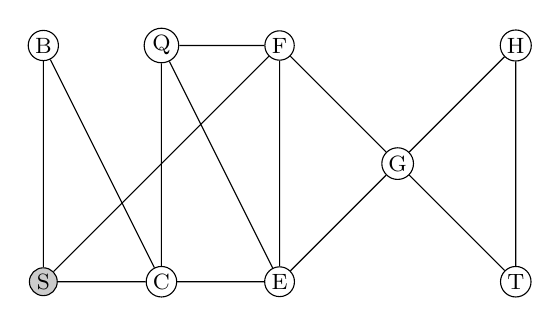
\begin{tikzpicture}[baseline=(current bounding box.center), xscale=.5]
\tikzstyle{every node}=[circle, draw, fill=black!0,
                        inner sep=1pt, minimum width=10pt, font = \footnotesize]
\path (0,0) node[fill=black!20] (A) {S} ;
\node (B)  at (0,3) {B};
\node (C) at (3,0) {C} ;
\node (E) at (6,0) {E} ;
\node (F) at (6,3)  {F} ;
\node (D) at (3,3)  {Q};
\node (G) at (9, 1.5) {G};
\node (H) at (12, 3) {H};
\node (I) at (12, 0) {T};
\draw (A) -- (B) -- (C) -- (D) -- (F);
\draw  (F)--(G) -- (E) -- (F);
\draw (D)-- (E) --(C) --(A)--(F);
\draw (H)--(I)--(G)--(H);
\end{tikzpicture}
%\end{center}
\end{adjustbox}
%
\begin{adjustbox}{valign=t,minipage={.25\textwidth}}

\begin{tabular}{ c | c | p{2in}}
Explored? & vertices & tentative distances\\ \hline
& \\
& \\
& \\& \\& \\& \\& \\& \\& \\% \\& \\& \\
 \end{tabular}


\end{adjustbox}

\begin{adjustbox}{valign=t,minipage={.25\textwidth}}
{
 \begin{tabular}{c | p{2in}}
vertex &  distance from $S$\\
\hline
S & \\ 
B & \\
C & \\ E & \\ F & \\ G & \\ H & \\ Q & \\ T & \\
\end{tabular}
}
\end{adjustbox}

\bigskip

What is the (shortest) distance between $S$ and $T$? \ans

\end{enumerate}

\end{document}

%-------------------------------------------------------------------------------------------------------------------------------------------------------------------------------------------------------------------

%%% Local Variables:
%%% mode: latex
%%% TeX-master: t
%%% End:
